\section{Results – Strategy S1: Single-Pass Full Input}
\label{sec:eval-s1}

The \textbf{S1: Single-Pass Full Input} configuration extracts all nine MUC-4 slots in a single LLM call. 
We evaluate three S1 variants: 
\textbf{S1.0} = no few-shot examples on the original MUC-4 dataset; 
\textbf{S1.1} = with few-shot examples on the original dataset; 
\textbf{S1.2} = with few-shot examples on a modified MUC-4 dataset that mimics speech-style transcripts.

\subsection*{Headline Results}


\begin{figure}[h]
\centering
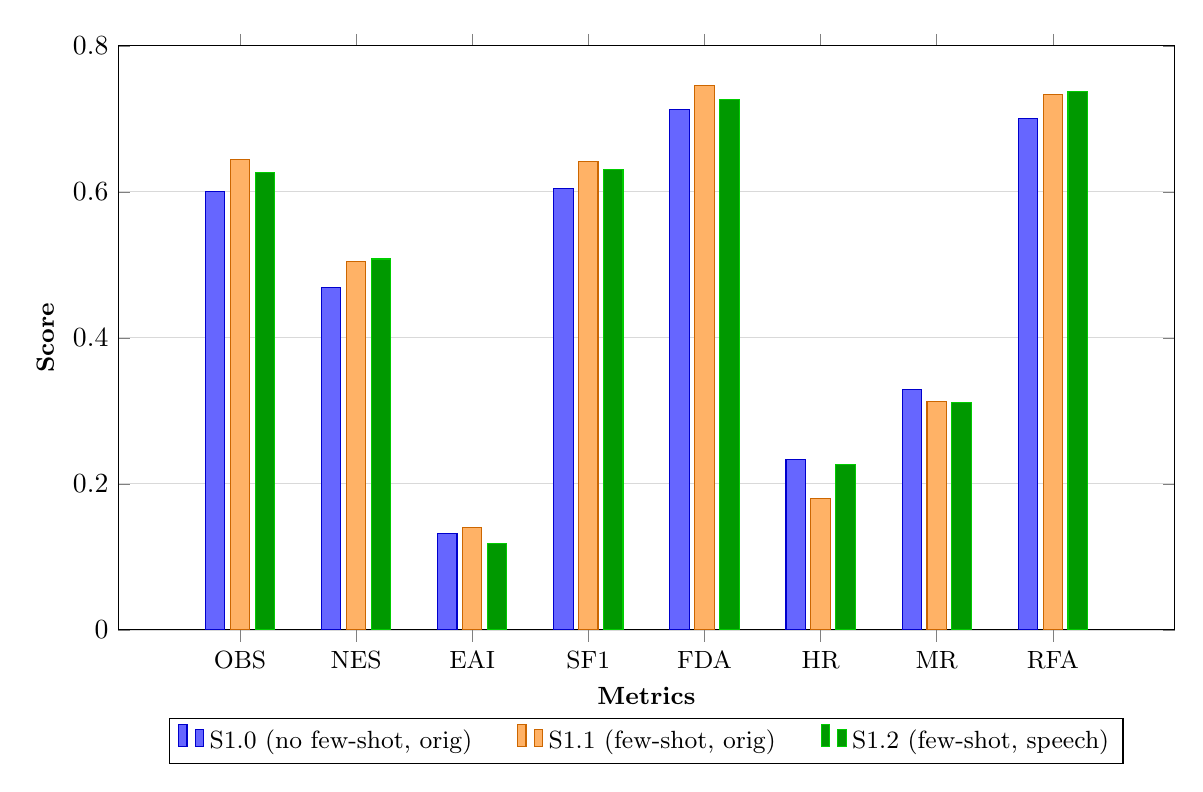
\begin{tikzpicture}
  \begin{axis}[
    width=15cm,
    height=9cm,
    ybar,
    bar width=7pt,
    ylabel={Score},
    ylabel style={font=\small\bfseries},
    xlabel={Metrics},
    xlabel style={font=\small\bfseries},
    symbolic x coords={OBS, NES, EAI, SF1, FDA, HR, MR, RFA},
    xtick=data,
    xticklabel style={font=\small},
    ymin=0,
    ymax=0.8,
    ytick={0, 0.2, 0.4, 0.6, 0.8},
    ymajorgrids=true,
    grid style={line width=0.3pt, draw=gray!30},
    legend style={
      at={(0.5,-0.15)},
      anchor=north,
      legend columns=3,
      font=\small,
      /tikz/every even column/.append style={column sep=0.5cm}
    },
    enlarge x limits=0.15,
  ]
  
  % S1.0 (no few-shot, orig) - Blue
  \addplot[fill=blue!60, draw=blue!80!black] coordinates {
    (OBS, 0.601)
    (NES, 0.469)
    (EAI, 0.132)
    (SF1, 0.604)
    (FDA, 0.713)
    (HR, 0.233)
    (MR, 0.329)
    (RFA, 0.700)
  };
  \addlegendentry{S1.0 (no few-shot, orig)}
  
  % S1.1 (few-shot, orig) - Orange
  \addplot[fill=orange!60, draw=orange!80!black] coordinates {
    (OBS, 0.644)
    (NES, 0.504)
    (EAI, 0.140)
    (SF1, 0.642)
    (FDA, 0.746)
    (HR, 0.180)
    (MR, 0.313)
    (RFA, 0.733)
  };
  \addlegendentry{S1.1 (few-shot, orig)}
  
  % S1.2 (few-shot, speech) - Green
  \addplot[fill=green!60!black, draw=green!80!black] coordinates {
    (OBS, 0.626)
    (NES, 0.508)
    (EAI, 0.118)
    (SF1, 0.631)
    (FDA, 0.727)
    (HR, 0.226)
    (MR, 0.311)
    (RFA, 0.738)
  };
  \addlegendentry{S1.2 (few-shot, speech)}
  
  \end{axis}
\end{tikzpicture}
\caption{Headline metrics for S1 variants on MUC-4 ($N{=}100$).}
\label{fig:s1-variants-bar}
\end{figure}

\paragraph{Per-field (reference for S1.1).}
\texttt{perpetratorOrganization} and \texttt{weapon} lead; \texttt{perpetratorIndividual} and \texttt{incidentLocation} remain harder.

\begin{table}[H]
    \centering
    \caption{Per-field average scores for S1.1 ($N{=}100$).}
    \label{tab:s1-perfield}
    \begin{tabular}{lcc}
        \toprule
        Field & Avg.\ Score & \#Docs \\
        \midrule
        incidentType & 0.510 & 100 \\
        incidentDate & 0.760 & 100 \\
        incidentLocation & 0.516 & 100 \\
        incidentStage & 0.710 & 100 \\
        perpetratorIndividual & 0.584 & 100 \\
        perpetratorOrganization & 0.752 & 100 \\
        target & 0.592 & 100 \\
        victim & 0.563 & 100 \\
        weapon & 0.807 & 100 \\
        \midrule
        \textbf{Overall (OBS)} & \textbf{0.644} & \textbf{900 comps} \\
        \bottomrule
    \end{tabular}
\end{table}

\subsection*{Latency}

\begin{figure}[H]
\centering
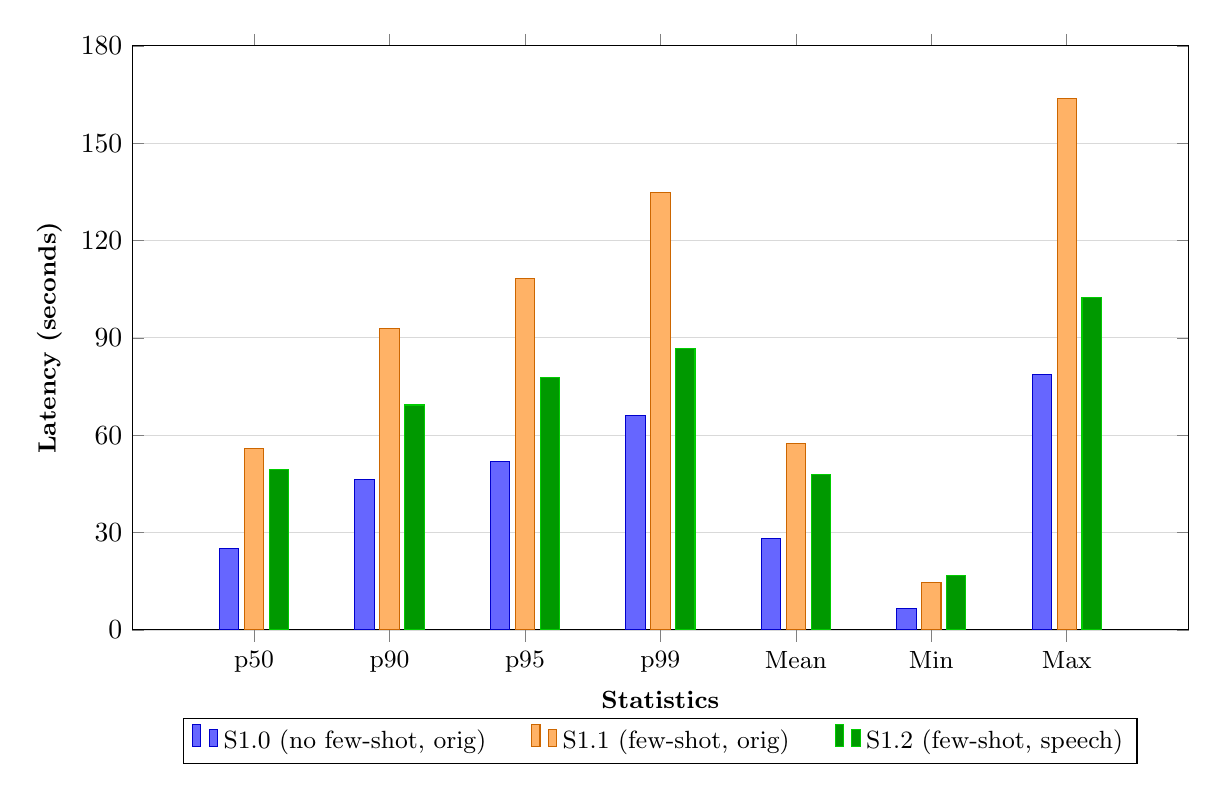
\begin{tikzpicture}
  \begin{axis}[
    width=15cm,
    height=9cm,
    ybar,
    bar width=7pt,
    ylabel={Latency (seconds)},
    ylabel style={font=\small\bfseries},
    xlabel={Statistics},
    xlabel style={font=\small\bfseries},
    symbolic x coords={p50, p90, p95, p99, Mean, Min, Max},
    xtick=data,
    xticklabel style={font=\small},
    ymin=0,
    ymax=180,
    ytick={0, 30, 60, 90, 120, 150, 180},
    ymajorgrids=true,
    grid style={line width=0.3pt, draw=gray!30},
    legend style={
      at={(0.5,-0.15)},
      anchor=north,
      legend columns=3,
      font=\small,
      /tikz/every even column/.append style={column sep=0.5cm}
    },
    enlarge x limits=0.15,
  ]
  
  % S1.0 (no few-shot, orig) - Blue
  \addplot[fill=blue!60, draw=blue!80!black] coordinates {
    (p50, 25.04)
    (p90, 46.49)
    (p95, 51.82)
    (p99, 66.12)
    (Mean, 28.17)
    (Min, 6.51)
    (Max, 78.65)
  };
  \addlegendentry{S1.0 (no few-shot, orig)}
  
  % S1.1 (few-shot, orig) - Orange
  \addplot[fill=orange!60, draw=orange!80!black] coordinates {
    (p50, 55.91)
    (p90, 93.01)
    (p95, 108.40)
    (p99, 134.93)
    (Mean, 57.34)
    (Min, 14.54)
    (Max, 163.79)
  };
  \addlegendentry{S1.1 (few-shot, orig)}
  
  % S1.2 (few-shot, speech) - Green
  \addplot[fill=green!60!black, draw=green!80!black] coordinates {
    (p50, 49.36)
    (p90, 69.30)
    (p95, 77.84)
    (p99, 86.79)
    (Mean, 47.89)
    (Min, 16.85)
    (Max, 102.50)
  };
  \addlegendentry{S1.2 (few-shot, speech)}
  
  \end{axis}
\end{tikzpicture}
\caption{Latency statistics for S1 variants (seconds).}
\label{fig:s1-latency-bar}
\end{figure}

\subsection*{Cost Analysis (S1: Single-Pass Full Input)}

\textbf{Assumptions.} Extraction on \textit{GPT-5} with $I{=}3{,}000$ input tokens and $O{=}300$ output tokens; verification on \textit{GPT-5-mini} with $V_{\text{in}}{=}1{,}000$, $V_{\text{out}}{=}100$. If audio is used, add Whisper transcription for $D$ minutes.

\textbf{Prices.} GPT-5: input \$1.25/M, output \$10.00/M. GPT-5-mini: input \$0.25/M, output \$2.00/M. Whisper: \$0.006/min.\footnote{OpenAI GPT-5 and GPT-5-mini pricing; Whisper API pricing. See OpenAI: \texttt{openai.com/gpt-5} and \textit{Introducing ChatGPT and Whisper APIs} (Apr 24, 2024).}

\textbf{Formula.}
\[
\text{Cost}=\frac{I}{10^6}p_{\text{in}}+\frac{O}{10^6}p_{\text{out}}
+\frac{V_{\text{in}}}{10^6}p^{(\text{mini})}_{\text{in}}
+\frac{V_{\text{out}}}{10^6}p^{(\text{mini})}_{\text{out}}
+0.006\cdot D
\]

\textbf{Per-record (no audio).}
\[
\underbrace{\tfrac{3000}{10^6}\!\cdot\!1.25}_{\$0.00375}
+\underbrace{\tfrac{300}{10^6}\!\cdot\!10.00}_{\$0.00300}
+\underbrace{\tfrac{1000}{10^6}\!\cdot\!0.25}_{\$0.00025}
+\underbrace{\tfrac{100}{10^6}\!\cdot\!2.00}_{\$0.00020}
=\mathbf{\$0.00720}\ (\approx 0.72\text{¢/doc})
\]
\textbf{With audio (Whisper).} Add $0.006\cdot D$. For $D{=}1$ min: $\$0.00720+0.006=\mathbf{\$0.01320}$ (\(\approx 1.32\,\text{¢}\)).
\textbf{Takeaway.} At these token sizes, S1’s LLM cost is $\sim\$0.0072$ per document; Whisper adds a simple linear \$0.006 per audio minute.


\subsection*{Insights}

\begin{itemize}
    \item \textbf{Few-shot boosts the single-pass baseline.} Moving from S1.0 to S1.1 improves OBS (+0.043) and SF1 (+0.038), increases FDA (0.713$\rightarrow$0.746), and cuts HR (0.233$\rightarrow$0.180). Gains concentrate in entity-rich fields (\texttt{perpetratorOrganization}, \texttt{weapon}) and reduce empty-field errors.
    \item \textbf{Speech-style inputs remain robust.} S1.2 trails S1.1 modestly on OBS/SF1 but achieves the best NES (0.508) and RFA (0.738), indicating strong content quality when gold is nonempty and both sides fill. Its lower EAI (0.118) suggests less dependence on empty-field advantage.
    \item \textbf{Decision behavior stabilizes with few-shot.} Few-shot lowers hallucination rate (HR) and raises fill-decision accuracy (FDA). S1.2 keeps FDA competitive (0.727) with the lowest missing rate (MR{=}0.311, tie within rounding), despite noisier inputs.
    \item \textbf{Consistent hard spots.} \texttt{perpetratorIndividual} remains the most difficult (sparse gold, high MR in nonempty regime); \texttt{incidentLocation} shows moderate improvements but stays challenging compared to \texttt{weapon}/\texttt{perpetratorOrganization}.
    \item \textbf{Latency–quality trade-off and overall choice.} S1.0 is fastest (p50 $\sim$25\,s/doc) but least accurate. S1.1 is the strongest accuracy baseline on clean text (p50 $\sim$56\,s/doc) at higher latency. S1.2 offers a middle ground for speech-like inputs—near S1.1 quality with shorter tails (p99 86.8\,s vs.\ 134.9\,s)—and is a sensible default when spoken-text robustness matters.
\end{itemize}
